\subsection*{\textcolor{subsectioncolor}{\textsf{3. \textit{SUBSYSTEM BREAKDOWN}}}}
\addcontentsline{toc}{subsection}{3. \textit{SUBSYSTEM BREAKDOWN}}

\begin{description}
\item[ClientSocket] berfungsi memastikan komunikasi dengan sisi \textit{server} berjalan sesuai protokol.
\item[DialogueManager] berfungsi menentukan apa yang selanjutnya akan diucapkan, dan juga yang akan dilakukan, seperti mengerjakan tugas dan/atau menyimpan informasi.
\item[FaceDetector] berfungsi melacak kedudukan muka pengguna.
\item[KnowledgeBase] berfungsi menulis masukan yang dianggap sebagai informasi yang harus diingat, dan membaca apa yang sudah tersimpan.
\item[NaturalLanguageAnalyser] berfungsi mencerna masukan.
\item[NaturalLanguageGenerator] berfungsi membentuk kalimat-kalimat dari apa yang akan dibicarakan.
\item[ServerSocket] berfungsi memastikan komunikasi dengan sisi \textit{client} berjalan sesuai protokol.
\item[SpeechRecogniser] berfungsi mengolah suara ucapan pembicara, baik untuk membuat teks darinya maupun untuk mengenali pembicara.
\item[SpeechSynthesiser] berfungsi menjadikan PUSPA dapat berbicara dengan suara.
\item[Synthespian] berfungsi menampilkan rupa karakter dengan segala pergerakannya.
\item[TaskManager] berfungsi mengolah perintah pengguna menjadi program (yang diluncurkan di \textit{server}) yang dapat menyelesaikan tugas yang bersangkutan.
\item[UserInterface] berfungsi sebagai antarmuka bagi pengguna saat menggunakan produk dengan cara-cara selain cara berbicara.
\end{description}

\subsubsection*{Diagram aliran kendali}
\includegraphics[width=0.3\textwidth]{DiagramAliranKendali}
